\chapter{Zhodnocení plynulosti pohybu}

	Nejen po dokončení, ale především i během debuggování řídícího systému jsem se snažil zhodnotit plynulost pohybu. Bohužel se mi nepodařilo dosáhnout očekávaných výsledků objektivních měření díky ne zcela vhodnému testovacímu stroji pro tato měření. Během debuggování jsem se tedy spoléhal na subjektivní hodnocení -- především na pohled, ale také i na poslech. Krokové motory totiž vydávají charakteristický zvuk dle svých otáček a jakékoliv cuknutí v~pohybu je tedy i slyšet.
	
	V~následujících podkapitolách popisuji způsob měření a výsledky. Veškeré výsledky se týkají nejnovější verze softwaru, která se nachází na přiloženém CD.
	
	Pro generování programů v~G-kódu jsem použil grafický program Inkscape s~pluginem GCodeTools\footnote{\url{http://www.cnc-club.ru/forum/viewtopic.php?t=35}}. Tento jednoduchý CAM program umožňuje generovat G-kód pro 2D vyřezávání a~gravírování, což pro mé potřeby debuggování plně dostačuje.

	\section{Subjektivní hodnocení}
	Pohyb testovacího plotteru řízeného mým interpolátorem vypadá na pohled plynule. O tom se lze přesvědčit na videích, která se nacházejí na přiloženém CD. I při dotyku rukou nejsou cítit žádné rázy. Jsou však cítit relativně silné vibrace. Tyto vibrace pocházejí od krokových motorů a jsou umocněny nepříliš tuhou konstrukcí a malou hmotností plotteru. Při umístění kilogramového závaží na pohyblivou plošinu plotteru jsou vibrace výrazně utlumeny.
	
	Při umístění skleničky s~vodou na plotter se hladina rozechvívá především díky vibracím. To usuzuji z~toho, že i při dlouhých pojezdech relativně malou rychlostí se na hladině objevují soustředné kruhové vlnky. Tehdy by se objevovat neměly, jelikož se jedná o pohyb rovnoměrný přímočarý. Při projíždění \uv{cik-cak čáry} jeví hladina jen malou tendenci se rozpohybovat a stále jsou mnohem výraznější vibrace od krokových motorů.
	
	\section{Objektivní měření}
	Abych ověřil funkčnost výpočtu rychlosti nejen subjektivně, ale také objektivně, rozhodl jsem se provést měření, která by funkčnost dokázala.
	
	\subsection{Měření na základě polohy}
	Jako první jsem chtěl z~interpolátoru odesílat zpět do počítače aktuální pozici jednotlivých os v~konstatním časovém intervalu. Na základě těchto dat jsem chtěl dopočítat aktuální rychlost, zrychlení a ryv. Běžně je pro grafické znázornění polohy na počítači použita zpráva {\tt STATEMESSAGE\_POSITION}. Tato zpráva se však dotazuje v~ne příliš přesném časovém rámci, což pro potřeby výše popsaného výpočtu nestačí.
	
	Periodu odesílání dat jsem zvolil 10~ms. Ačkoliv jsem odesílal pouze pozici os x a~y, tedy dohromady 8 bytů, narazil jsem na propustnost rozhraní USB, resp. limity integrované periférie v~mikroprocesoru či způsobu vyčítání dat na počítači. Interpolátor přestal stíhat interpolovat a aplikace na počítači přestávala reagovat. Ani paketizace dat (kdy jsem posíl větší množství dat naráz) nepomohla. Příčinu této relativně malé propustnosti se mi nepodařilo zjistit, ačkoliv při dřívějších testech přenosová rychlost opačným směrem (z~počítače do mikrokontroléru) dosahovala několika Mbit$\cdot$s$^{-1}$ 
	
	\subsection{Měření pomocí akcelerometru}
	Dále jsem se pokusil změřit působící zrychlení na plotteru pomocí integrovaného MEMS akcelerometru v~mobilním telefonu. Měření jsem prováděl na mobilní telefonu Nokia Lumia 920. Tento telefon jsem vybral, jelikož ze~všech pro mě dostupných telefonů má nejnižší hladinu šumu výstupu z~akcelerometru. Od tohoto měření jsem si nesliboval žádné výsledky, prováděl jsem je pro zajímavost. O to více mě překvapily výsledky tohoto měření.
	
	Pro telefon jsem napsal jednoduchou aplikaci, která s~nejvyšší možnou frekvencí (u~mnou použitého telefonu to je 66~Hz) vyčítá data z~akcelerometru. Tato zaznamenaná data jsem si díky relativně omezenému způsobu přístupu k~paměti v~systému Windows Phone 8 posílal pomocí e-mailu do počítače. Telefon byl k~plotteru pevně připevněn pomocí modelářských svorek (obrázek \ref{obr:met1}).
	
	\begin{figure}[h]
		\centering
		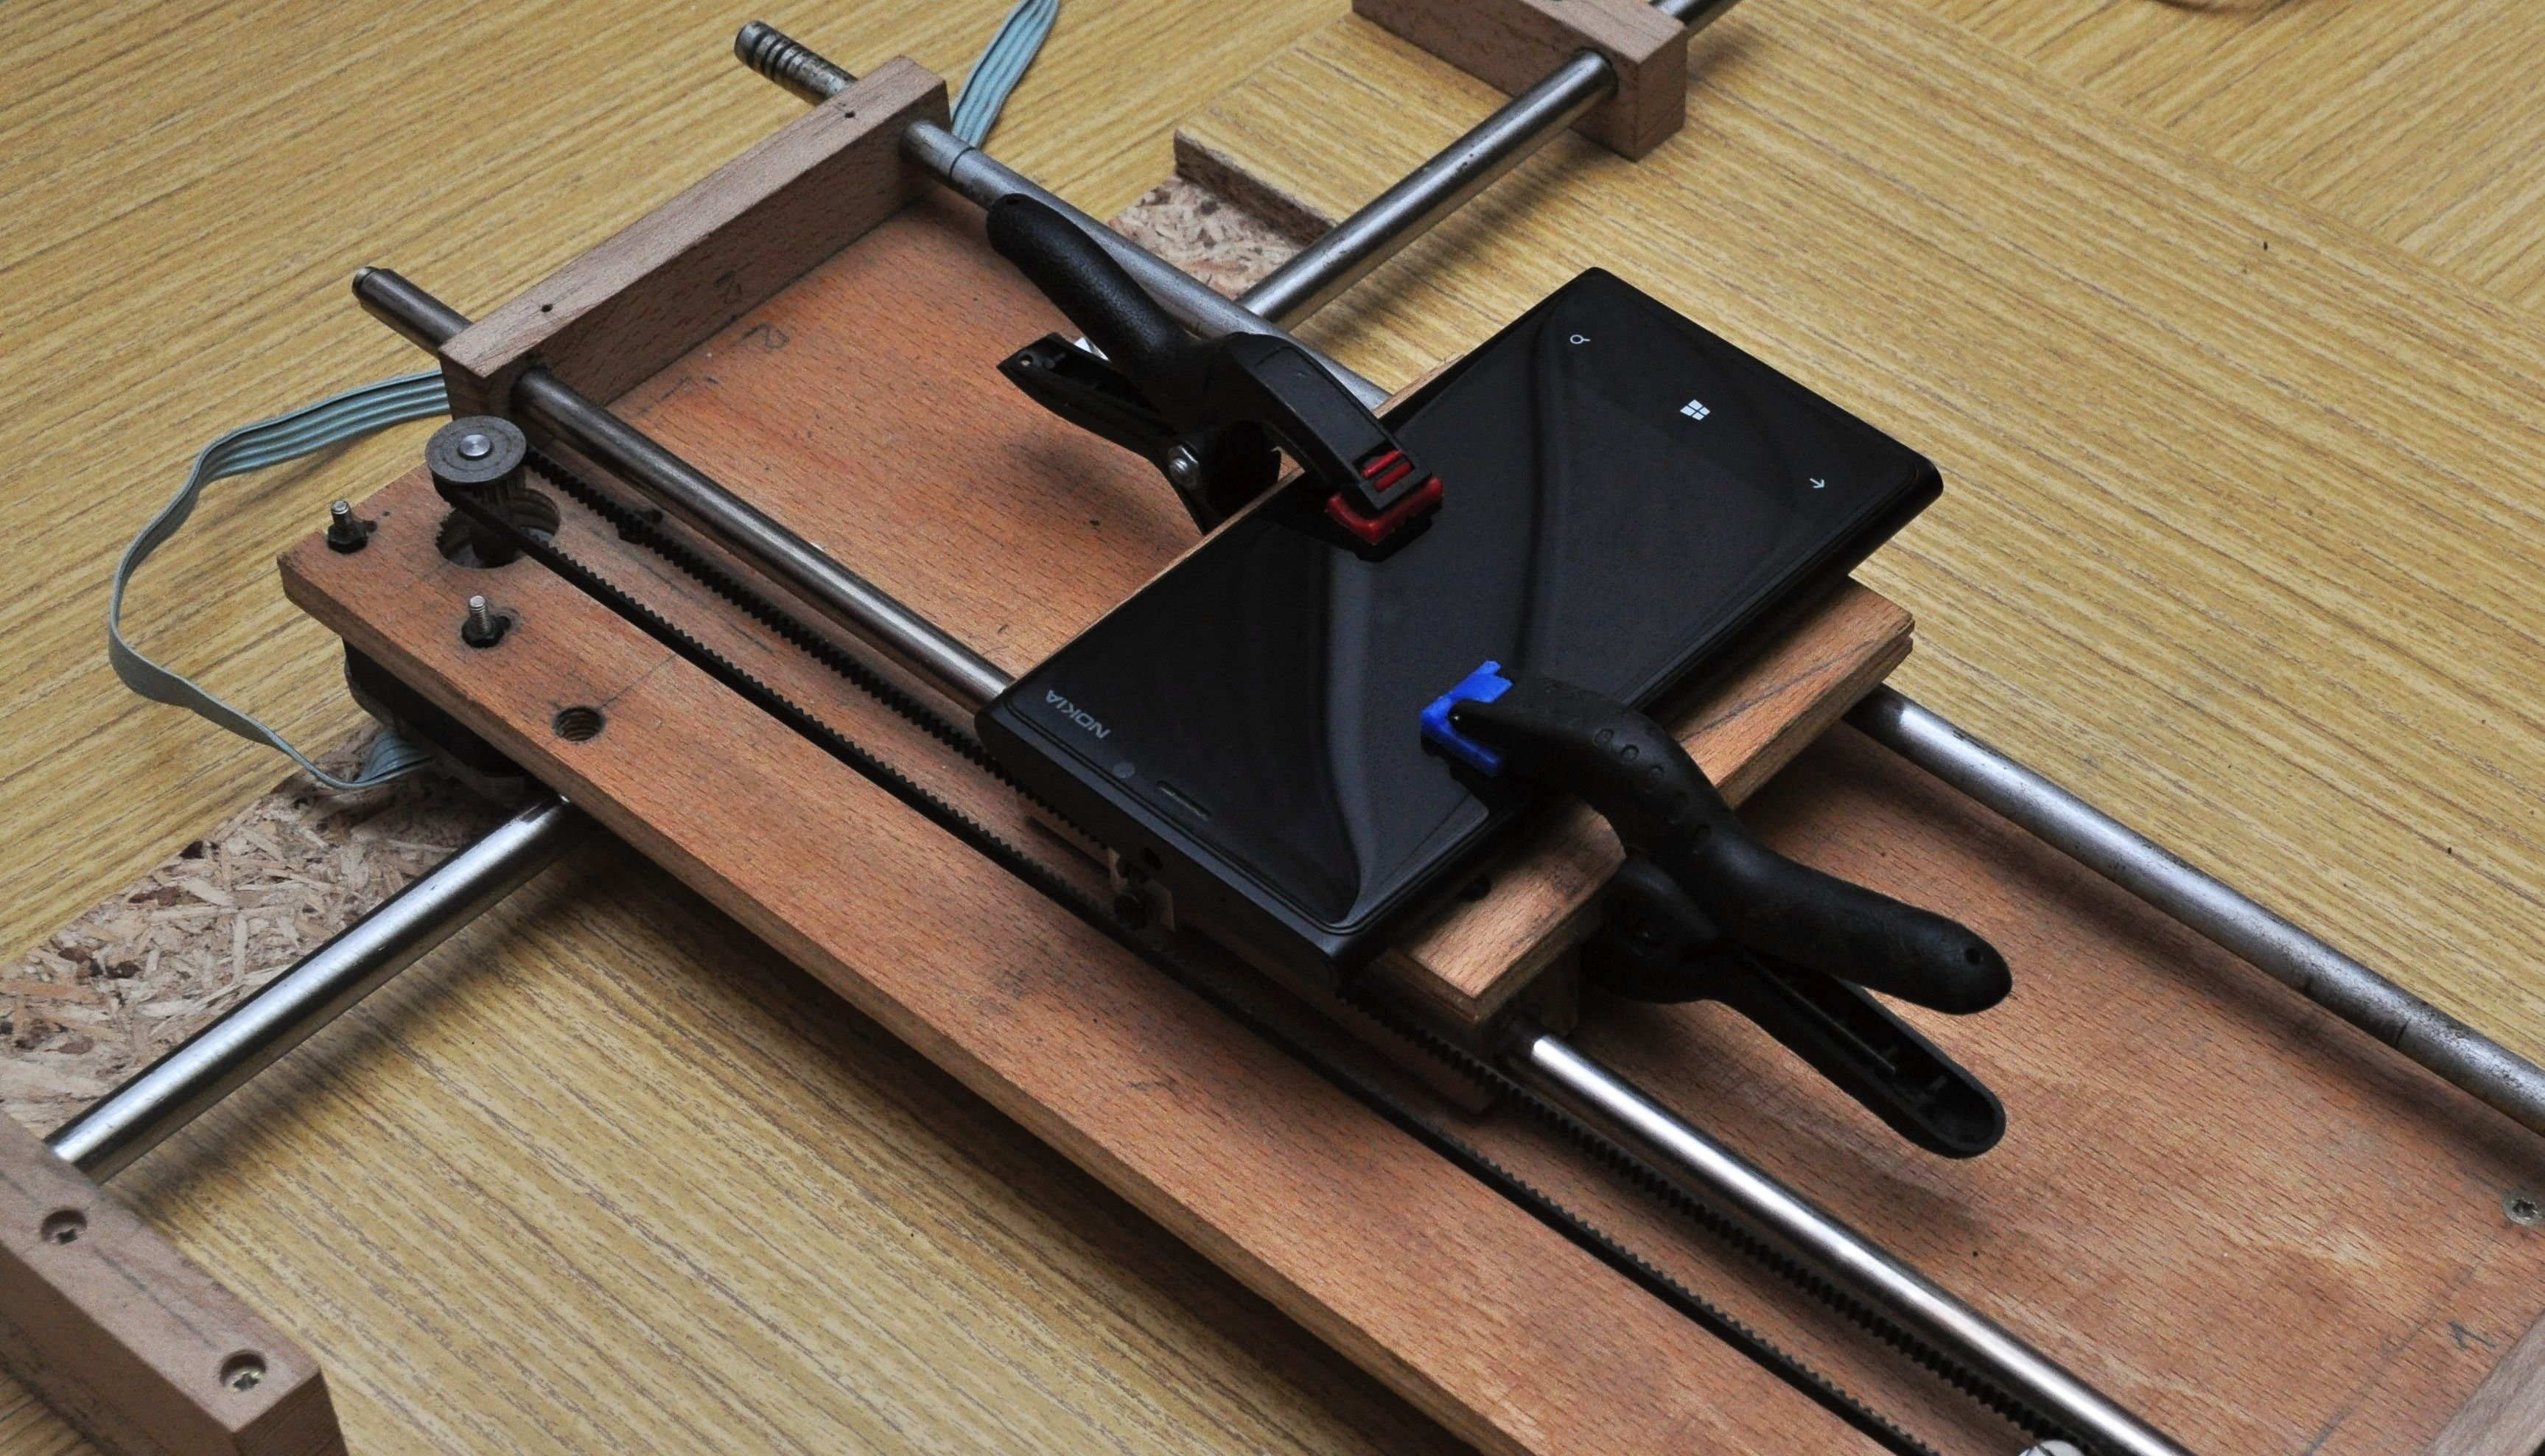
\includegraphics[width=0.9\textwidth]{img/metodika1.jpg}
		\caption{Metodika měření zrychlení pomocí akcelerometru.}\label{obr:met1}	
	\end{figure}
	
	Pro vyčtení dat z~akcelerometru jsem použil dva způsoby. První způsob využívá Motion API\footnote{\url{http://msdn.microsoft.com/en-us/library/windowsphone/develop/hh202984(v=vs.105).aspx}}. Toto API poskytuje informace o~poloze telefonu založené na všech dostupných senzorech. Pro má měření jsem využíval člen {\tt DeviceAcceleration} struktury {\tt MotionReading}. Tento člen poskytuje trojrozměrný vektor vyjadřující veškerá zrychlení působící na telefon s~odečtením tíhového.
	
	Druhý způsob využíval třídu {\tt Accelerometer} ze jmeného prostoru {\tt Microsoft.Devices.Sensors}\footnote{\url{http://msdn.microsoft.com/en-us/library/windowsphone/develop/ff431810(v=vs.105).aspx}}. Tato třída poskytuje přímo data z~akcelerometru. Abych získal informace o pohybu, uložil jsem si v~klidovém stavu telefonu vektor působícího tíhového zrychlení, a následně jsem jej při každém měření odečítal od vektoru všech působících zrychlení. Tím jsem dostal pouze vektor zrychlení způsobující pohyb.
	
	Ačkoliv jsem od druhého způsobu očekával přesnější výsledky, ukázala se data vyčtená oběma způsoby jako téměř rovnocená.
	
	Data jsem získal z~následujícího programu v~G-kódu:
	\begin{verbatim}
		G00 X0 Y0 Z0.000000
		G01 X100 F2500
		G01 Y20
		G01 X0 Y0
	\end{verbatim}
	Tento program zobrazuje trojúhelník. První částí pohybu je 100~mm dlouhý posun pouze osou~x rychlostí 2500~mm$\cdot$min$^{-1}$ (přibližně 42~mm$\cdot$s$^{-1}$). Druhá část je 20~mm dlouhý posun pouze osou~y. Následně se plotter vrátí do výchozích souřadnic -- nastvá pohyb obou os. Maximální amplituda zrychlení byla nastavena na 4000~mm$\cdot$s$^{-2}$ a maximální ryv na 8000~mm$\cdot$s$^{-3}$.
	
	Mnou naměřená data jsou zobrazena na grafu \ref{graf:nefiltr}. Jelikož jsou tato data nepřehledná, zkusil jsem vyfiltrovat -- každou hodnotu jsem vzal jako průměr dvou předcházejících a dvou nadcházejících prvků. Tato vyfiltrovaná data jsou zobrazena na grafu \ref{graf:filtr}. Na těchto datech jsou silně patrné vibrace od krokových motorů. Na datech lze spatřit vykonávaný pohyb, ale nelze je prohlásit za 100\% průkazná.
	
	Mezi časy $t=0,6~$s a $t=2,8~$s lze vidět 100mm pohyb osou x. V~čase 0,6 sekundy se nachází výrazný peak zrychlení na ose~x -- to je zrychlení nutné pro dosažení požadované rychlosti. Tento peak je jasně vidět, jelikož plotter byl v~klidu a nenastaly na něm žádné vibrace. V~čase 2,8 sekundy lze vidět peak na ose~x s~opačnou amlitudou. To je zpomalování na konci pohybu. Výchylka pro zrychlení odpovídá svou velikostí nastaveným hodnotám. Výchylka pro zpomalení je o něco menší -- to si vysvětluji jako nepřenost měření způsobenou vibracemi. K~těmto peakům na ose~x lze najít i stejně široké malé peaky na ose~y. Jejich existenci si vysvětluji nepřesným upevněním telefonu, kdy měřící osa~x v~akcelerometru nebyla uložena zcela rovnoběžně s~osou~x na plotteru. Mezi těmito dvěma peaky probíhá pohyb rovnoměrný přímočarý a naměřené zrychlení je způsobeno vibracemi od plotteru.
	
	V grafech již nelze vypozorovat pohyb podél osy~y. Zde předpokládám, že vyčtení znemožnily silné vibrace. Osa~y se totiž nachází na portálu, v~němž je upevněn její motor. Tento portál poté s~motorem rozonuje. Portál je také pevně uložen v~pozdrech na vodicí tyči pouze na jedné straně -- na druhé straně po vodicí tyči klouže (kdyby byl uložen pevně i na druhé straně, musela by být naprosto přesně seřízena rovnoběžnost vodicích tyčí). Motor je navíc uložen na klouzající straně, čímž se celá situace ještě zhoršuje. Na ose~x nejsou tyto vibrace tak silné, jelikož je pevně spojena se základnou a je celkově tužší.

	
	\begin{figure}[h!]	
		\centering
		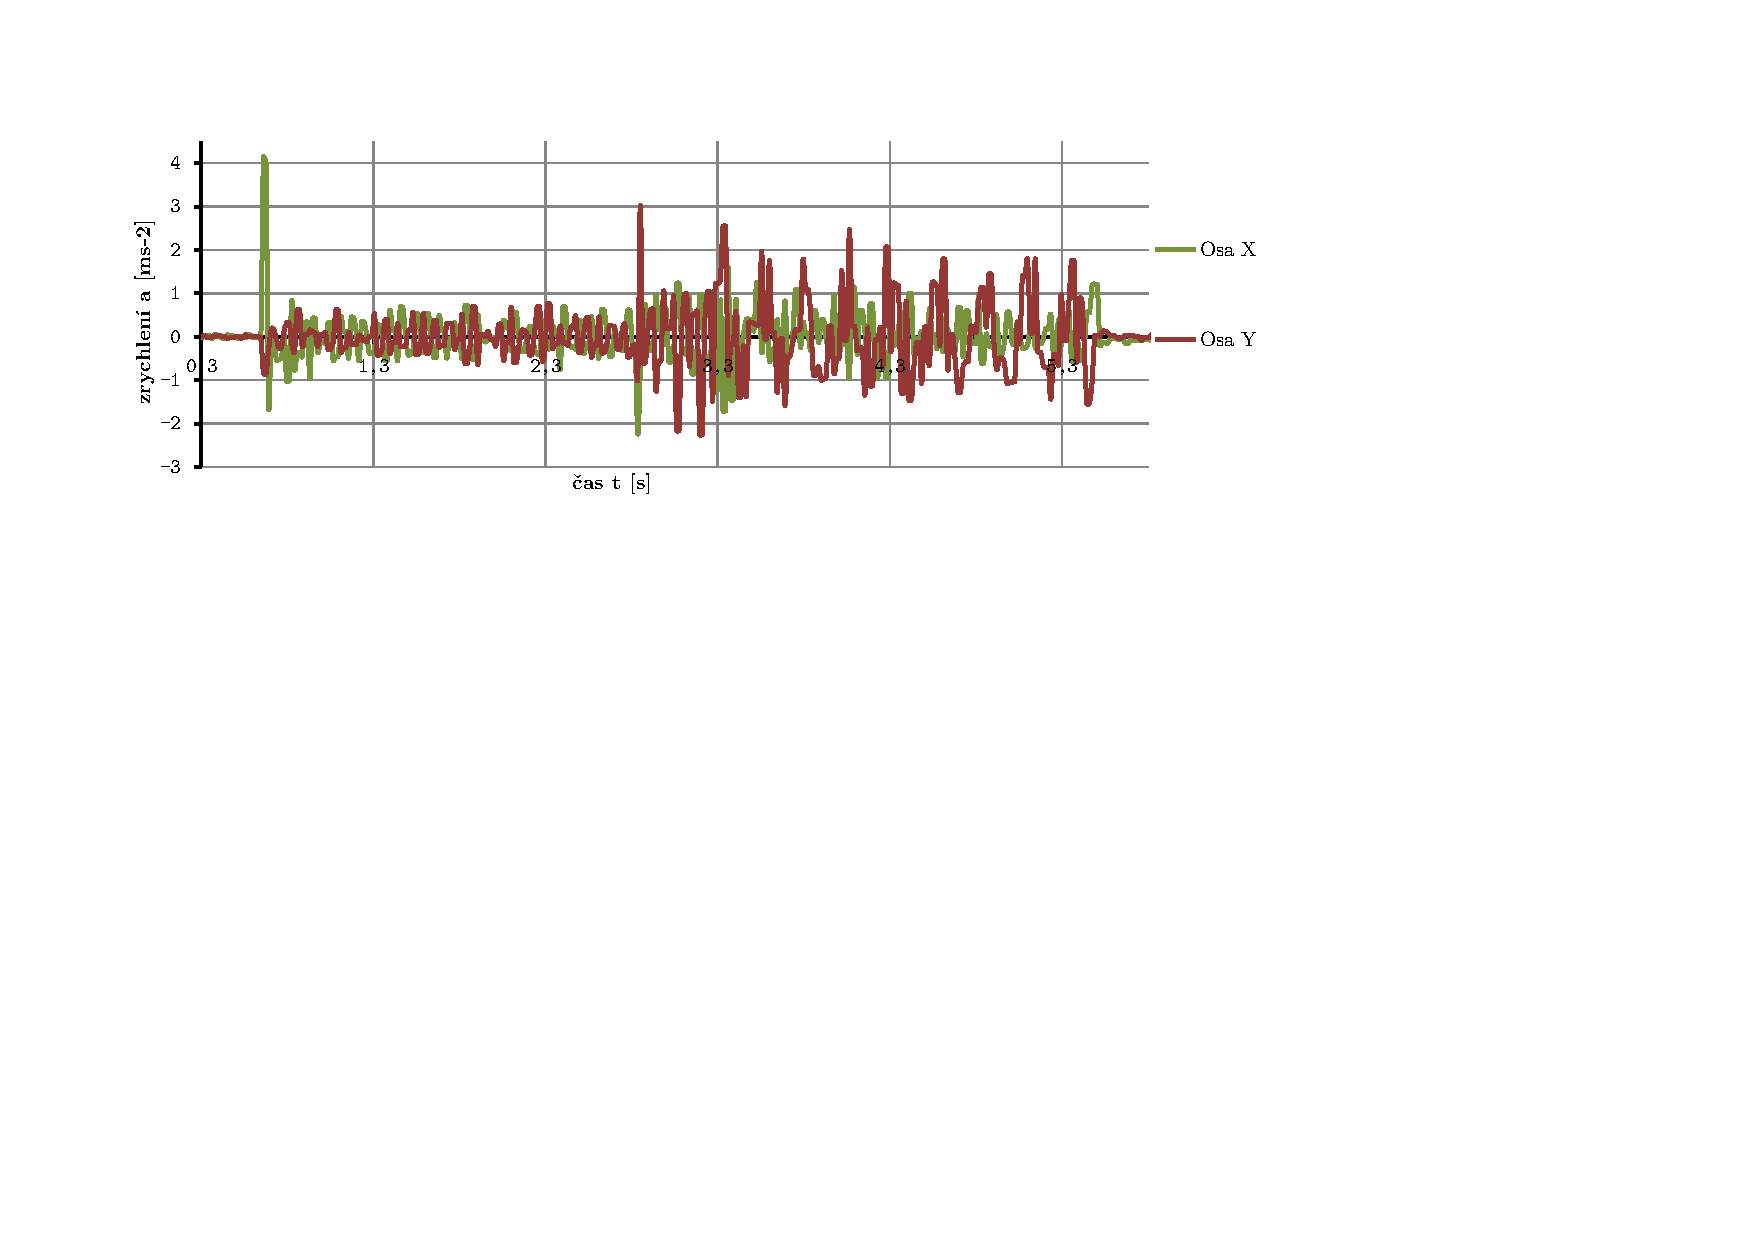
\includegraphics[width=\textwidth]{img/nefiltrovane.pdf}
		\caption{Naměřená data z akcelerometru.}\label{graf:nefiltr}	
	\end{figure}
	
	\begin{figure}[h!]	
		\centering
		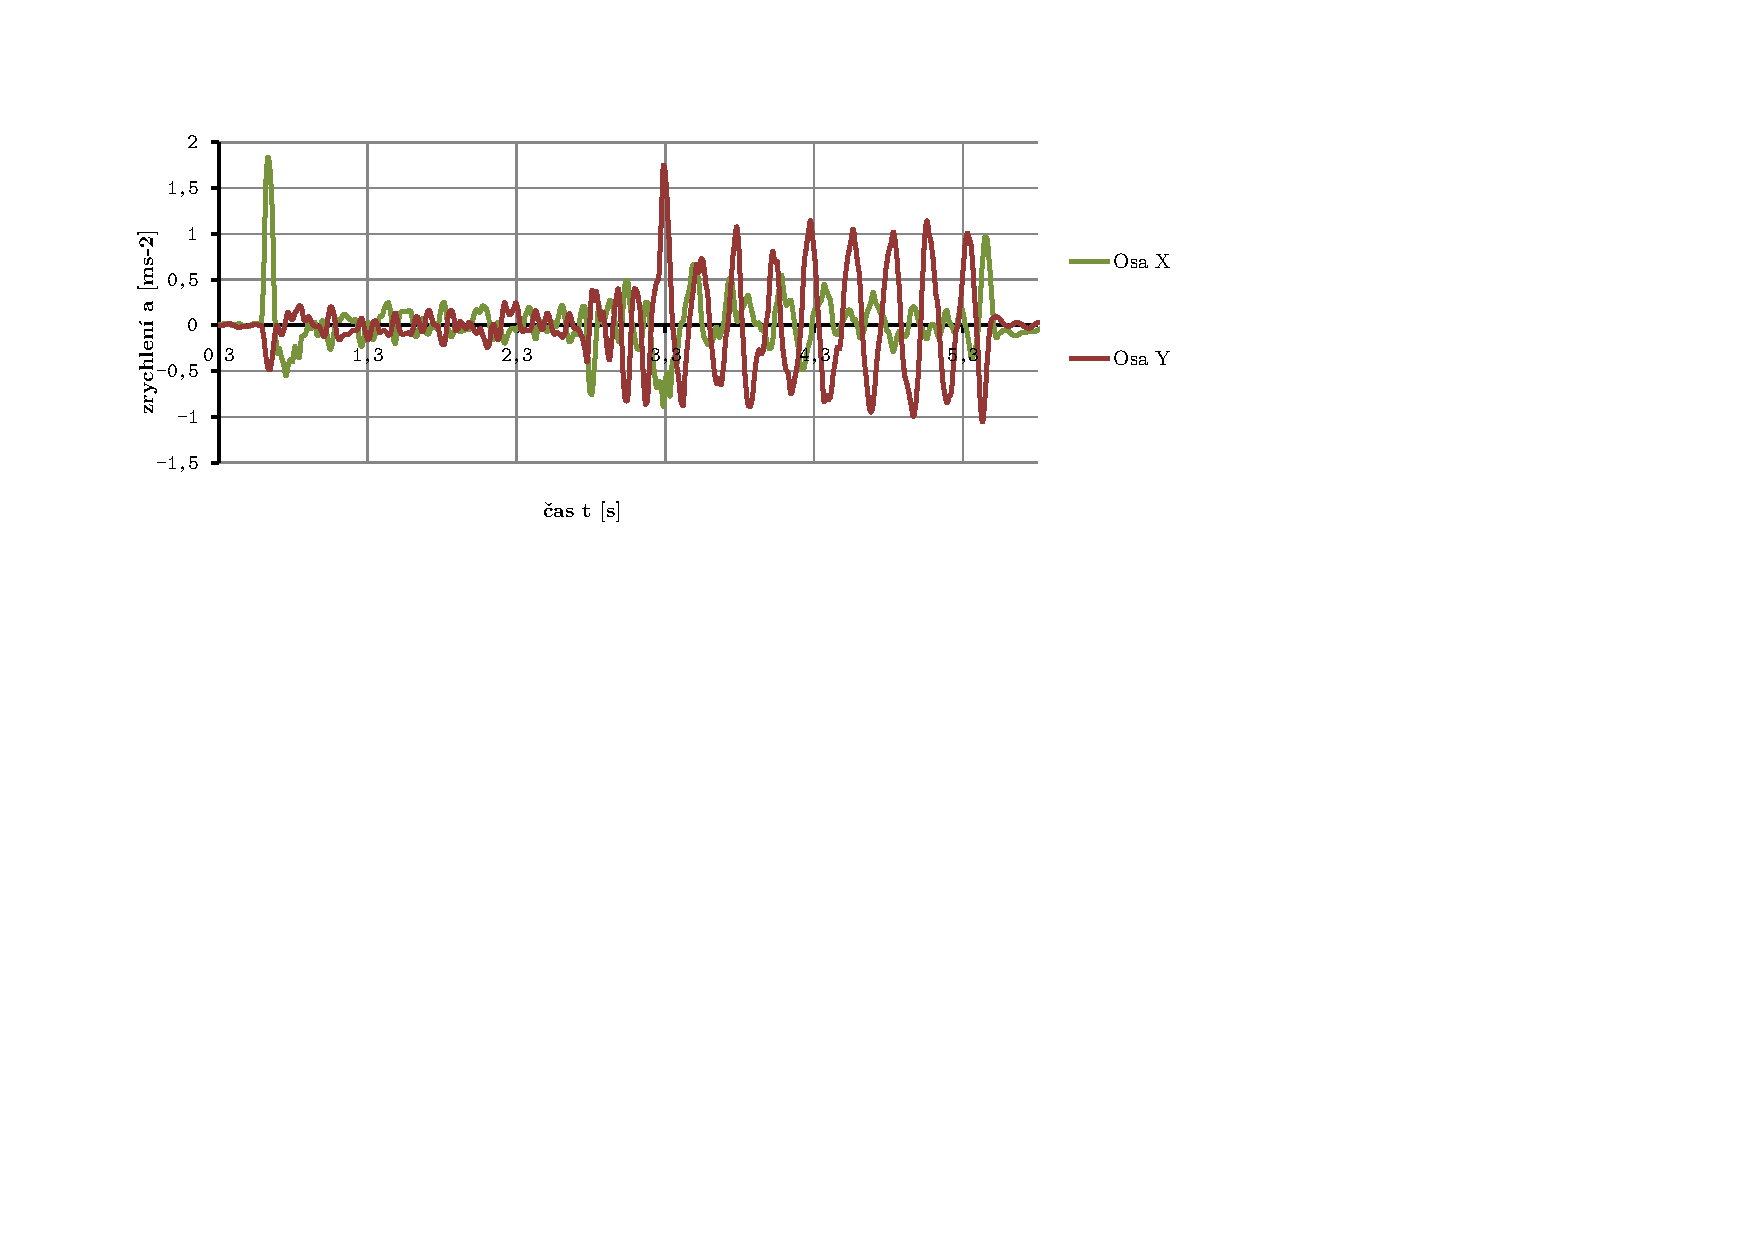
\includegraphics[width=\textwidth]{img/filtrovane.pdf}
		\caption{Filtrovaná data z grafu \ref{graf:nefiltr}}\label{graf:filtr}	
	\end{figure}
	
	Jelikož první měření poskytla relativně slibné výsledky, rozhodl jsem se upravit metodiku měření a pokusit se získat průkaznější data. Vibrace konstrukce jsou obrovským problémem, a tak jsem se rozhodl pohyblivou část plotteru zatížit 1,5kg závažím, na které jsem upevnil telefon. Telefon jsem tentokrát společně se závažím připevnil k~plotteru pomocí několika pevně utažených gumiček. Od závaží jsem očekával utlumení vibrací a~připevnění gumičkou jsem zvolil, abych zamezil přímému přenosu vibrací (obrázek \ref{obr:met2}).
	
	\begin{figure}[h]
			\centering
			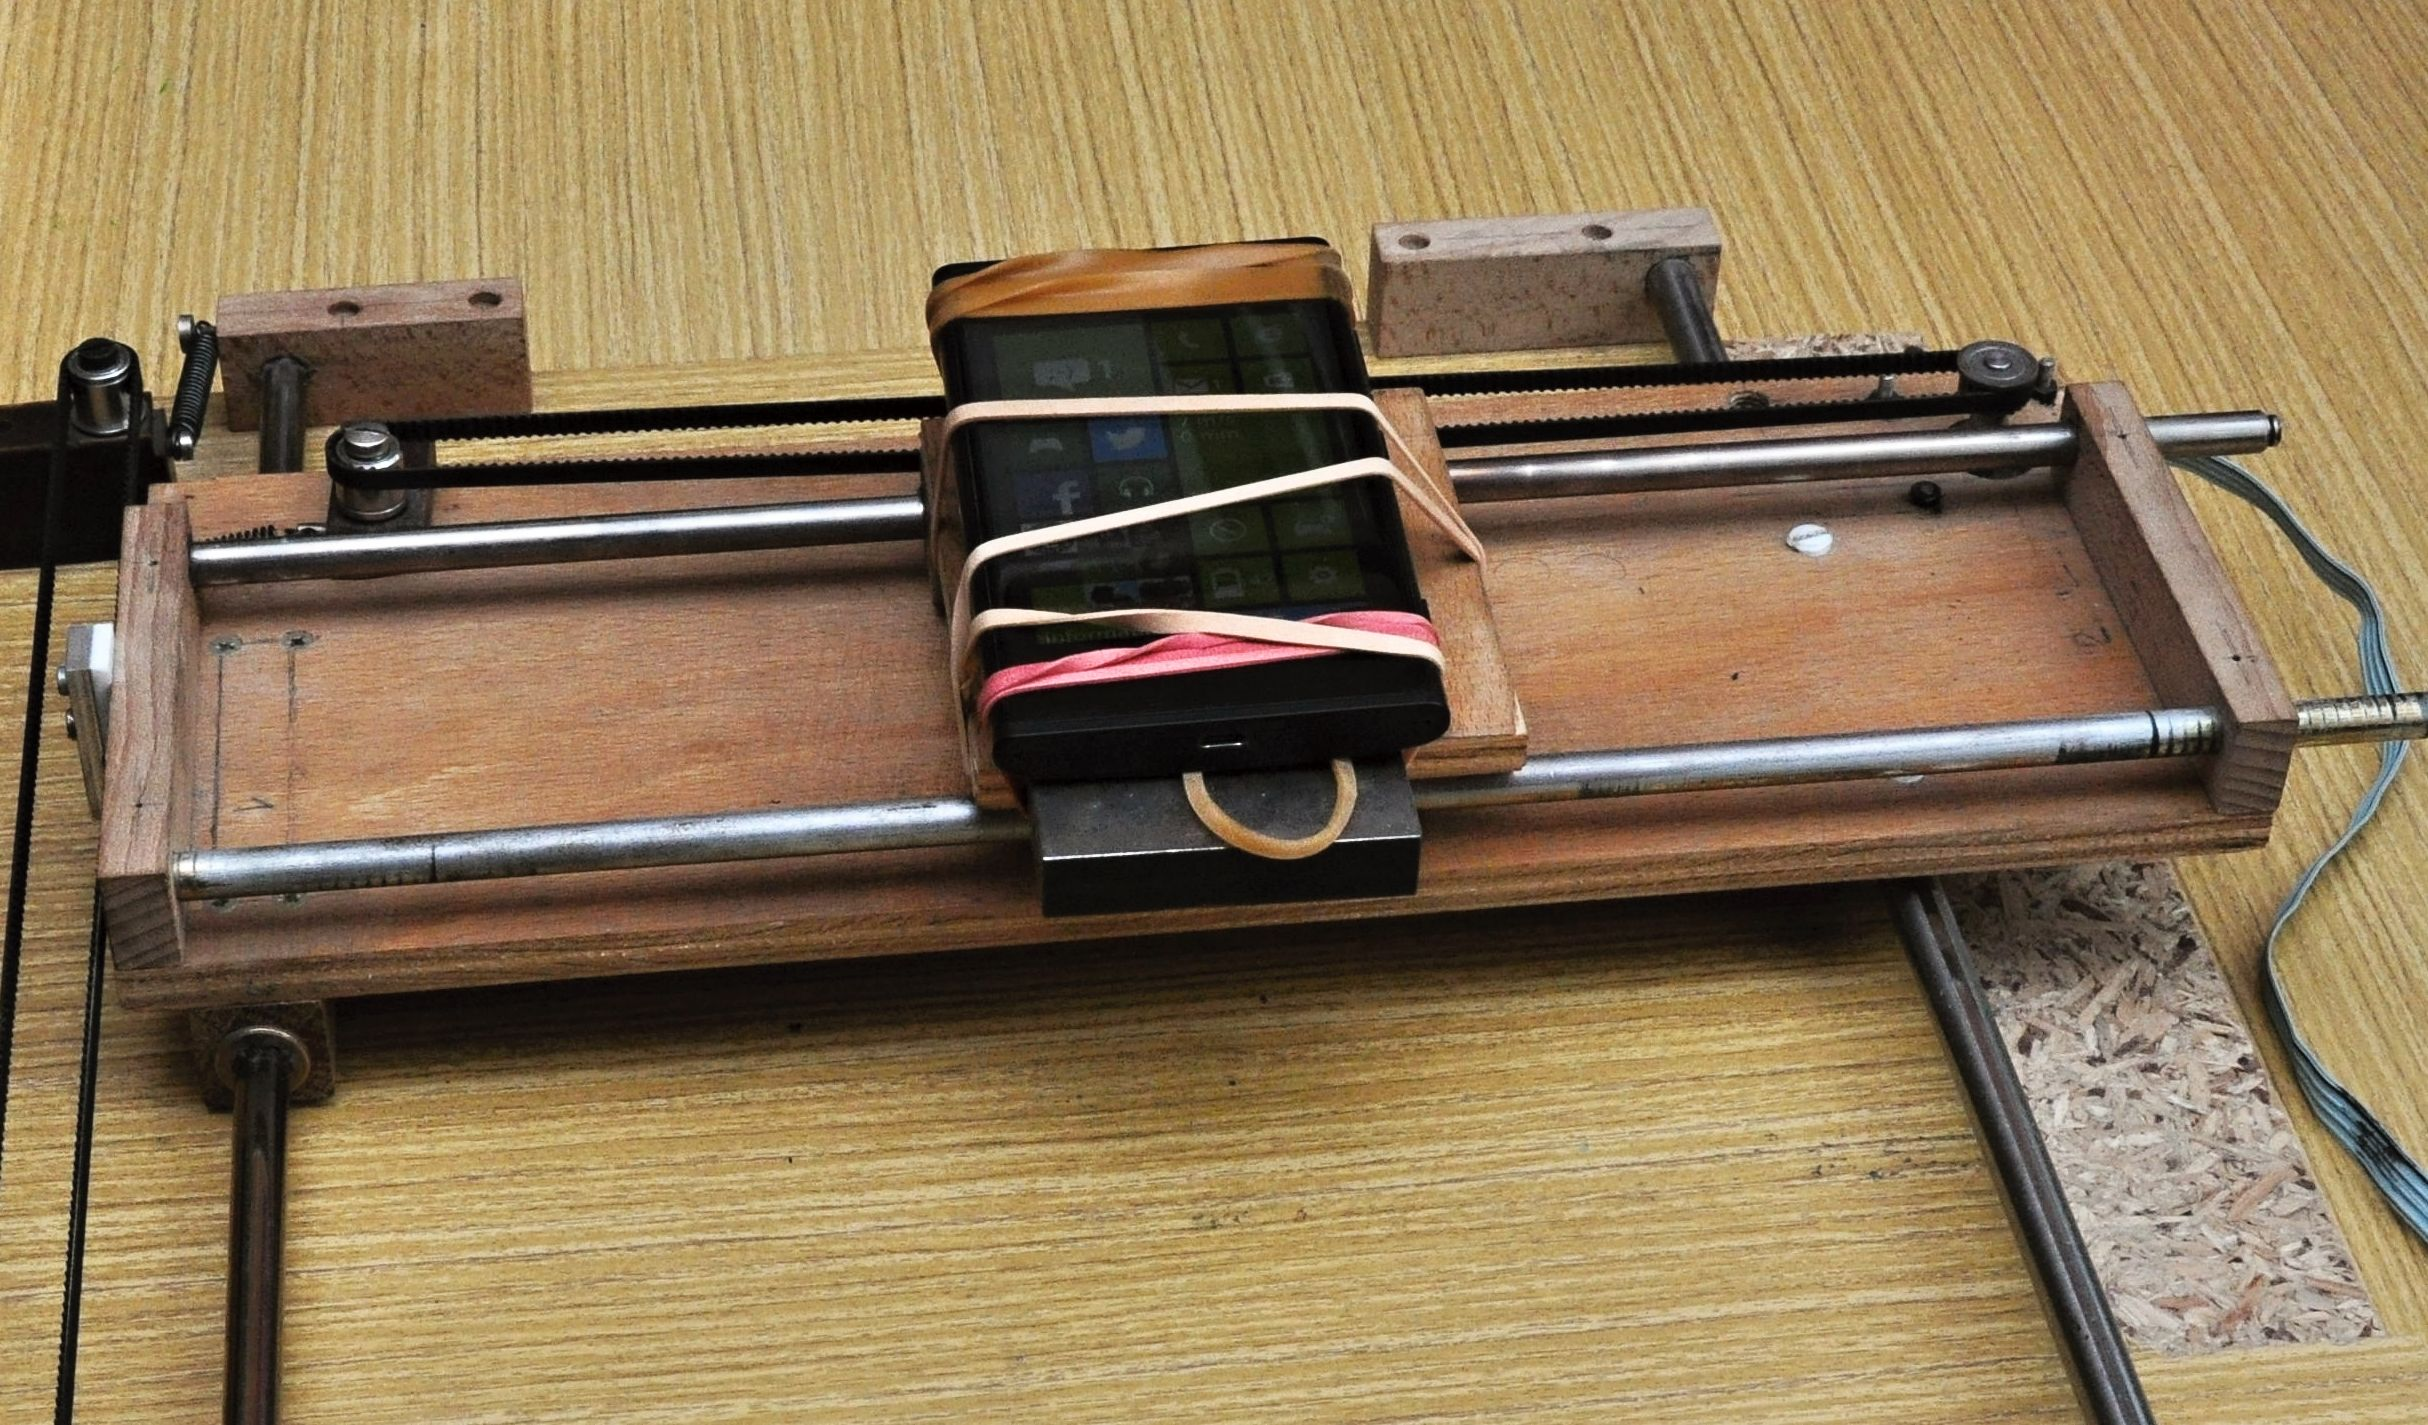
\includegraphics[width=0.7\textwidth]{img/metodika2.jpg}
			\caption{Nové uchycení telefonu pro měření zrychlení.}\label{obr:met2}	
	\end{figure}
	
	Výsledky mých měření jsou zobrazeny na grafech \ref{graf:nefiltr2} a~\ref{graf:filtr2}. Data byla vyfiltrována stejně jako v~prvním případě. Má očekávání se naplnila. Vibrace byly znatelně utlumeny, jak lze vidět na vyfiltrovaném grafu. Jasně je rozpoznatelné počáteční zychlení na začátku pohybu ve směru osy~x (v~čase 2,5~s), dobře je vidět zrychlení i při pohybu ve směru osy~y a~také je vidět dobře konečné brzdění (v~čase 7~s). Toto brzdění má zápornou amplitudu o téměř stejné velikosti jako rozjezd.
	
	V~naměřených datech je však jeden úsek, který si neumím vysvětlit -- mezi 4. a~5. sekundou by mělo probíhat brzdění při pohybu ve směru osy~x. Jenže zde se nenachází žádné zrychlení se zápornou amplitudou. Nevím, čím si tuto chybu v~měření vysvětlit. Pravděpodobně se jedná o nějaké propružení použitého upevnění telefonu. Na grafu je opět vidět vibrace při pohybu na ose~y, avšak jejich amplituda je mnohem menší.
	
	Z tohoto druhého měření je vidět, že systém funguje tak, jak má. I přesto by bylo zajímavé jej přeměřit pomocí lepších prostředků.
	
	\begin{figure}[h]	
			\centering
			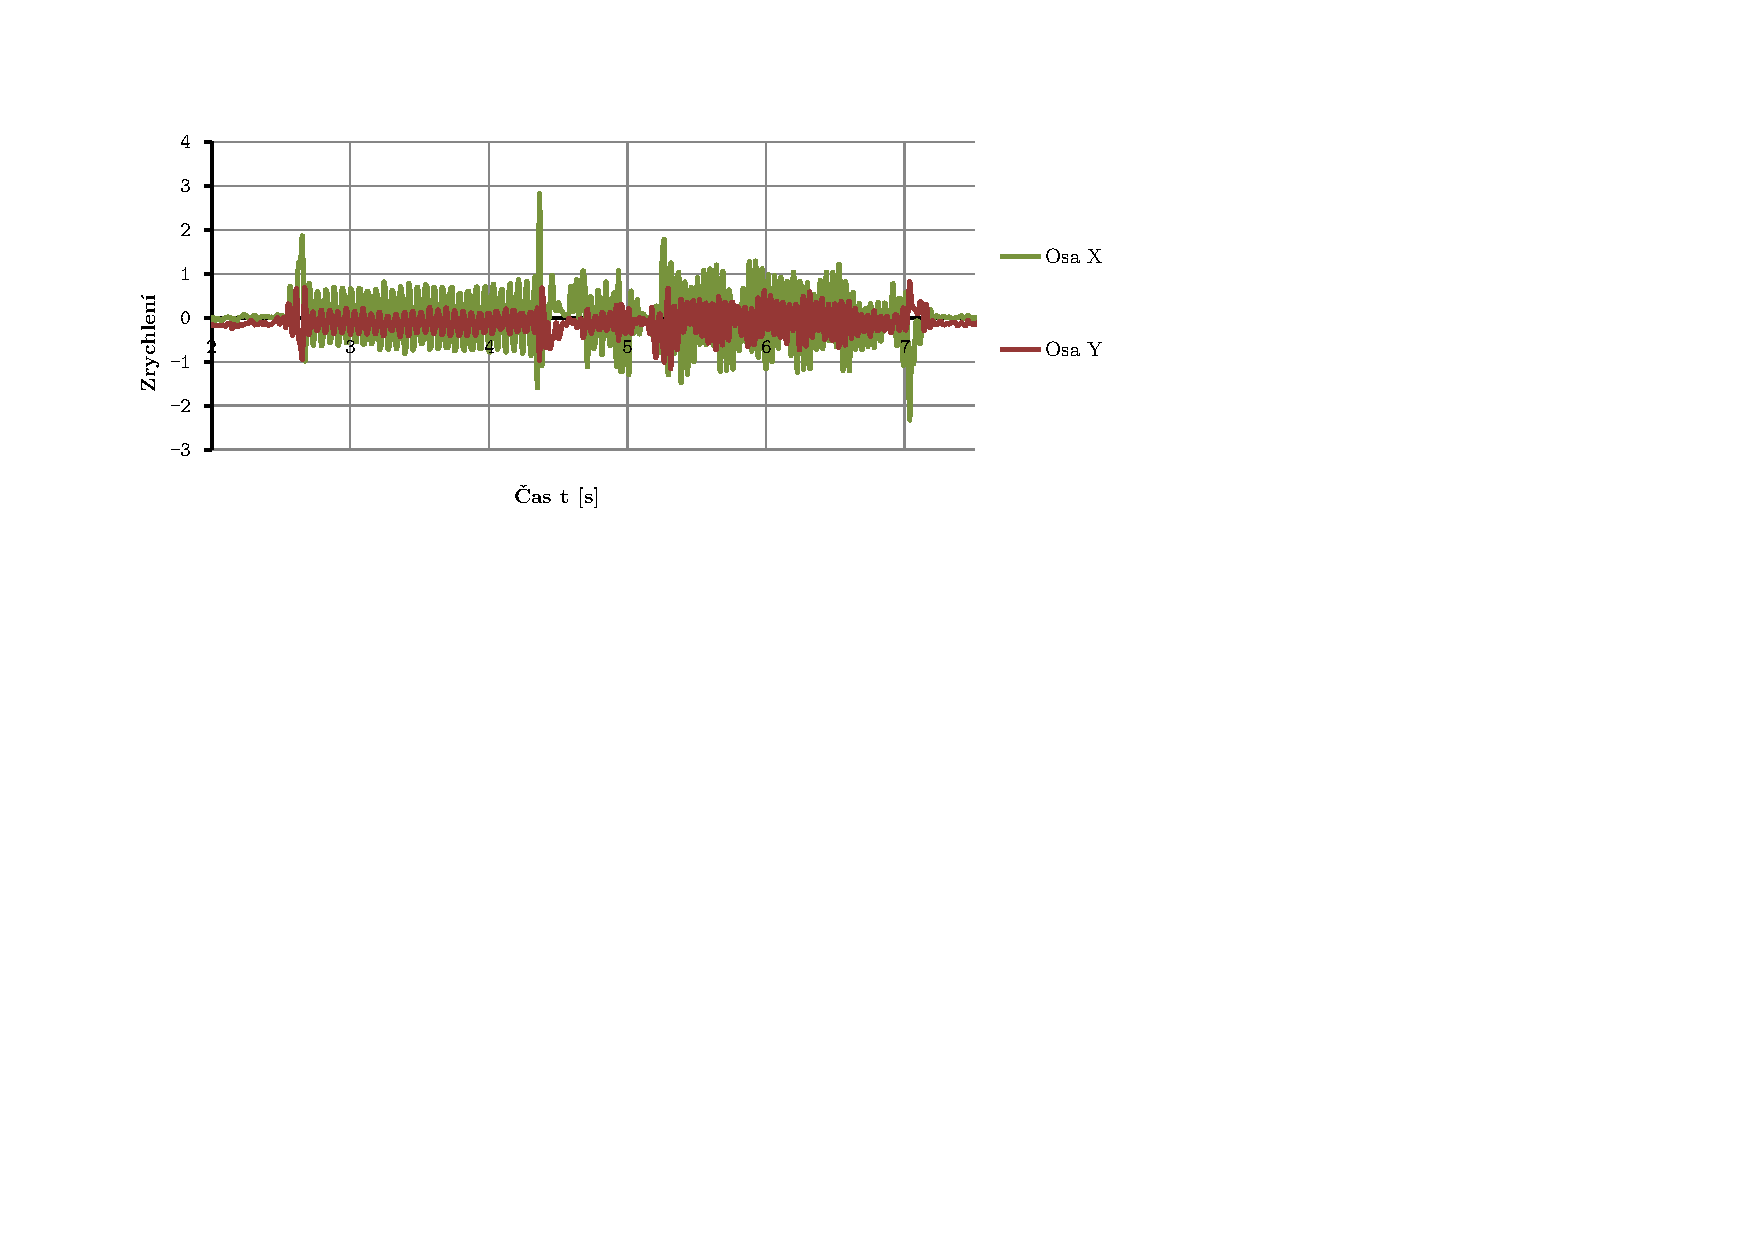
\includegraphics[width=\textwidth]{img/nefiltrovane2.pdf}
			\caption{Naměřená data z akcelerometru.}\label{graf:nefiltr2}	
		\end{figure}
		
		\begin{figure}[h]	
			\centering
			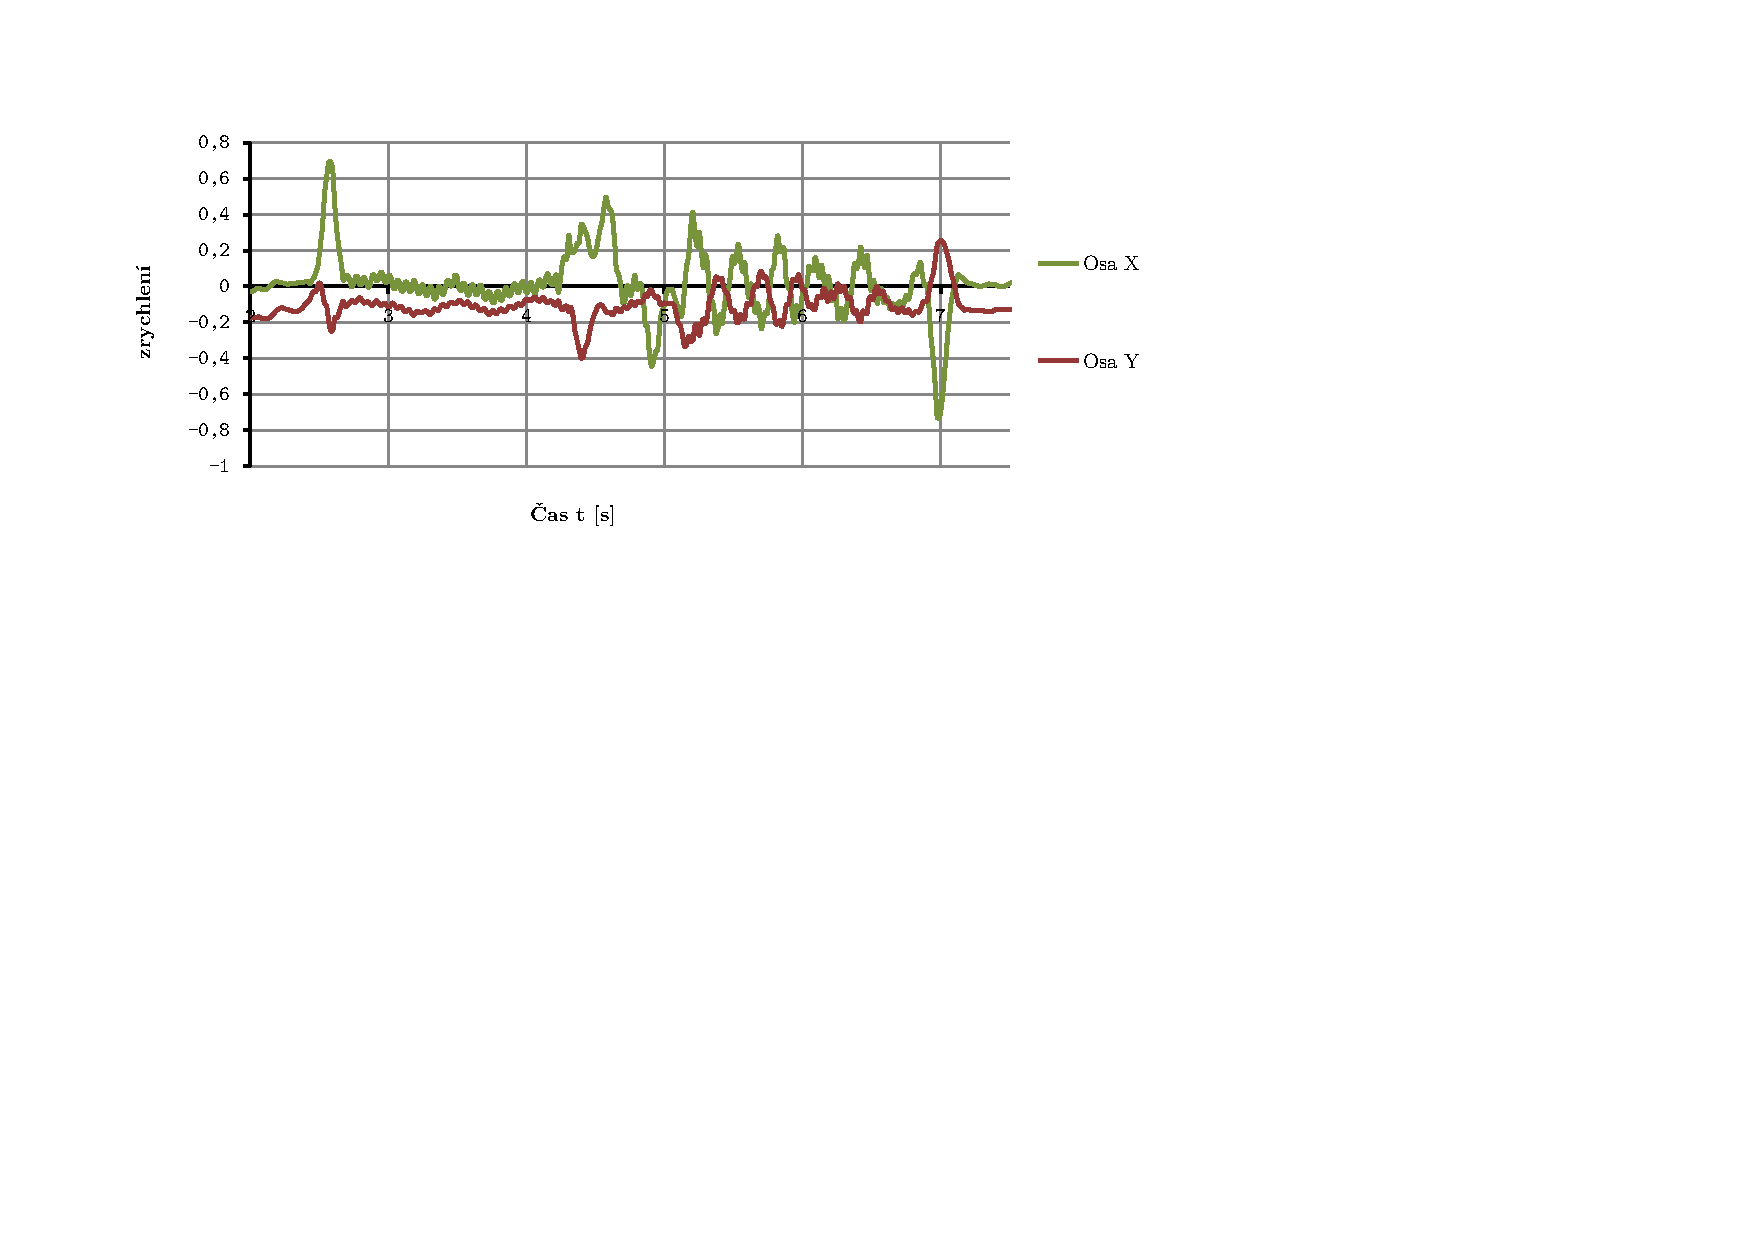
\includegraphics[width=\textwidth]{img/filtrovane2.pdf}
			\caption{Filtrovaná data z grafu \ref{graf:nefiltr2}}\label{graf:filtr2}	
		\end{figure}
	
\chapter{Současný stav projektu a~jeho budoucnost}

Můj řídicí systém ve své současné verzi umí načítat G-kód s~podporou pro většinu běžně používaných G-kódů (jejich seznam je uveden v~tabulce \ref{tab:funkce}). Dále je schopen provádět kompenzaci nástroje. Systém zvládá určit a~poté i následně interpolovat pohyb po akceleračních S-křivkách s~omezením jak maximálního přípustného zrychlení, tak i maximálního ryvu. Tento výpočet zvládá jak pro lineární, tak i obloukový pohyb. Interpolační výkon jednotky je dostatečný na to, aby byla schopna interpolovat pohyb posuvy i kolem 10--15~m$\cdot$min$^{-1}$.

Můj systém se však nyní nachází spíše v~podobě technického dema než skutečného projektu/produktu. Ačkoliv zvládá ty nejpodstatnější úlohy, postrádá spoustu drobné funkcionality, která by mu umožnila být nasazen přímo v~praxi. Z~této drobné funkcionality můžu jmenovat podporu limitní snímačů, tabulku nástrojů, pokročilé ovládání programu (navazování po přerušení), podpora pro vřeteno a~vlastně i samotné provedení interpolátoru. Můj systém ve své současné podobě slouží jako demonstrace možností řízení pohybu CNC stroje z~pohledu dynamiky. Ukazuje funkčnost mnou odvozeného fyzikálního modelu, ukazuje jeho přednosti, ale není vhodý pro nasazení do praxe.

Dříve jsem byl optimističtější a~plánoval jsem např. nahrazení počítače tabletem, což by umožnilo pohodlnější zabudování systému do stroje (aplikace pro tablet existuje, avšak je ve stádiu pokusů -- zatím je schopna pouze zpracovávat jednoduchý G-kód bez podpory korekce nástroje). Avšak s~postupem času se ukázalo, jak časově náročné by bylo doplnění veškeré nutné funkcionality. Rozhodl jsem se tedy projekt ponechat ve stádiu technického dema.

Z původních cílů tohoto projektu se mi povedlo splnit téměř všechny. Podařilo se mi navrhnout a~odvodit vhodný fyzikální model pro pohyb CNC stroje. Také se mi povedlo realizovat interpolační jednotku, která obstarává úkony náročné na časování a~počítač používá pouze pro uživatelský vstup a~výkonově náročné operace. Dále se mi povedlo realizovat USB komunikaci mezi jednoutkou a~počítačem. Jediný cíl, kterého jsem nedosáhl, je nasazení jednotky do praxe.

Ačkoliv jsem se rozhodl opustit můj projekt ve stádiu technického dema, zvažuji, zda-li by nestálo za to zaimplementovat můj fyzikální model do již existujícího řídícího systému. Tento systém by poskytl robustní základ pokrývající veškerou nutnou funkcionalitu. Jako vhodný se jeví řídicí systém LinuxCNC, který je opensource\cite{linuxcnc}, ale chybí mu propacovanější model práce s~dynamikou stroje. Nezkoumal jsem však možnosti této úpravy a~už vůbec ne složitost tohoto úkonu. Tato myšlenka je pouze ve stádiu úvahy.